% -*- TeX -*-
\documentclass{beamer}

\usepackage{amsmath}
\usepackage{array}
\usepackage{tikz}

\usetikzlibrary{decorations.pathreplacing}
\usetikzlibrary{fit,matrix}

\title{Crustal Deformation Modeling Tutorial}
\subtitle{Using Gravity and Initial Stresses}
\author{Charles Williams \\
  Brad Aagaard \\
  Matthew Knepley}
\institute{
\includegraphics[scale=0.4]{../../logos/cig_blackfg}}
\date{June 27, 2017}


% ---------------------------------------------------- CUSTOMIZATION
\renewcommand{\thispdfpagelabel}[1]{}
\newcommand{\pylith}[1]{{\color{green}#1}}
\newcommand{\python}[1]{{\color{red}#1}}
\usetheme{CIG}

\newcommand{\tensor}[1]{\overline{#1}}

% ========================================================= DOCUMENT
\begin{document}

% ------------------------------------------------------------ SLIDE
\maketitle

% ------------------------------------------------------------ SLIDE
\logo{
\includegraphics[height=4.5ex]{../../logos/cig_blackfg}}

% ========================================================== SECTION
\section{Gravitational body forces}

% ========================================================== SUBSECTION
\subsection{Concepts covered}
% ------------------------------------------------------------ SLIDE
\begin{frame}
  \frametitle{Concepts Covered in this Session}
  \summary{}

  \begin{itemize}
  \item When are gravitational stresses necessary?
  \item Usage of gravitational body forces in 3D
  \item Usage of initial stresses
  \item Usage of small strain formulation in 3D
  \item Viscoelastic relaxation with a linear Maxwell model
  \item Spatial database with irregular distribution of points in 3D
  \end{itemize}

  \vfill
  NOTE:  Accuracy and convergence for gravitational problems will be
  much improved once PyLith includes higher-order elements.
  \vfill
  
\end{frame}


% ========================================================== SUBSECTION
\subsection{When is gravity needed?}

% ------------------------------------------------------------ SLIDE
\begin{frame}
  \frametitle{When Do We Need to Use Gravitational Stresses?}
  \summary{}

  \begin{itemize}
  \item Pressure/stress-dependent rheology
    \begin{itemize}
    \item Pressure-dependent bulk rheology (e.g., plasticity)
    \item Stress-dependent fault rheology (e.g., friction)
    \end{itemize}
  \item Viscoelastic simulations where we care about vertical
    deformation
  \item Other simulations where we care about the absolute stress
    state
  \end{itemize}
  
\end{frame}


% ========================================================== SECTION
\subsection{Other examples}

% ------------------------------------------------------------ SLIDE
\begin{frame}
  \frametitle{Other Gravity Examples}
  \summary{}

  \begin{itemize}
  \item 2-D examples: {\tt\color{red} examples/2d/gravity}
  \begin{itemize}
    \item Steps 1-3: Body forces, initial stresses, infinitesimal strain
      \begin{itemize}
      \item Step 1: Body forces + infinitesimal strain
      \item Step 2: Body forces + infinitesimal strain + initial stress
      \item Step 3: Step 2 + local density variation
      \end{itemize}
    \item Steps 4-7: Body forces, initial stresses,
      finite/infinitesimal strain with postseismic relaxation
      \begin{itemize}
      \item Step 4: Relaxation with infinitesimal strain and no gravity
      \item Step 5: Relaxation with finite strain and no gravity
      \item Step 6: Relaxation with infinitesimal strain and gravity
      \item Step 7: Relaxation with finite strain and gravity
      \end{itemize}
    \item Step 8: Usage of initial state variables and density
      variation
    \end{itemize}
  \item 3-D examples: {\tt\color{red} examples/3d/hex8/step15-17}
  \end{itemize}
  
\end{frame}


% ========================================================== SECTION
\subsection{Cascadia gravity examples}

% ------------------------------------------------------------ SLIDE
\begin{frame}
  \frametitle{Cascadia Gravity Simulations}
  \summary{}

  \vfill
  Files are in {\tt\color{red} examples/3d/subduction}
  None of these problems involve faulting.
  \vfill

\begin{enumerate}
\item {\tt\color{red} step08a} Use gravitational body forces for an
  elastic problem and balance them with initial stresses computed for a
  constant mantle density.
  \begin{itemize}
  \item Stresses are out of balance and there is significant
    deformation.
  \end{itemize}
\item {\tt\color{red} step08b} Use gravitational body forces for an
  elastic problem and balance them with initial stresses from
  {\tt\color{red} step08a}.
  \begin{itemize}
  \item Stresses are in balance and there is no deformation.
  \end{itemize}
\item {\tt\color{red} step08c} Use gravitational body forces for a
  viscoelastic problem with finite strain and balance them with the same
  initial stresses as for {\tt\color{red} step08b}.
  \begin{itemize}
  \item Stresses are in balance for the elastic solution but viscous
    flow in the time-dependent solution results in large deformations.
  \end{itemize}
\end{enumerate}

\end{frame}


% ========================================================== SECTION
\subsection{Step 8a}

% ------------------------------------------------------------ SLIDE
\begin{frame}
  \frametitle{Step 8a}
  \summary{Elastic infinitesimal strain with initial stress from
    mantle density}

  \vfill
  \begin{center}
      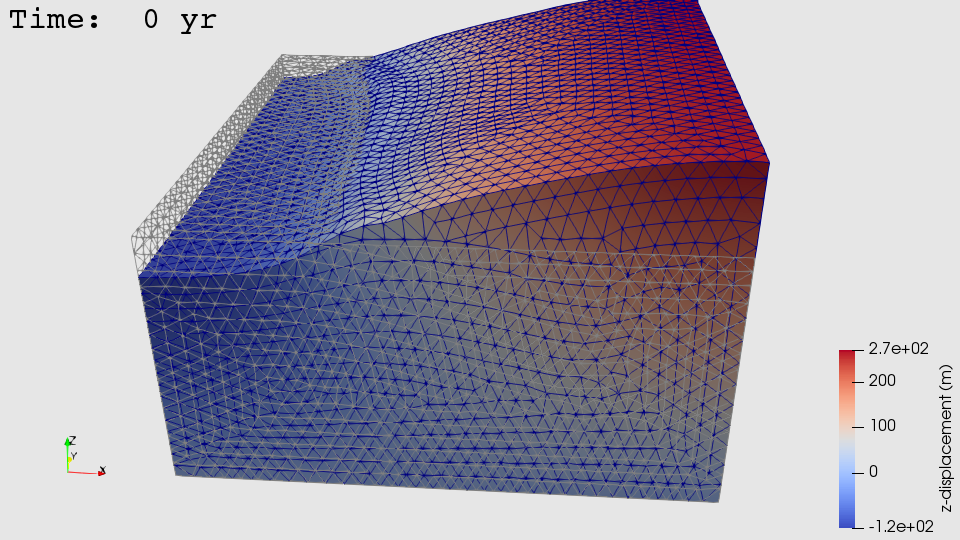
\includegraphics[height=6.1cm]{figs/subduction3d_step08a_soln}
  \end{center}
\vfill
      
\end{frame}


% ========================================================== SECTION
\subsection{Step 8b}

% ------------------------------------------------------------ SLIDE
\begin{frame}
  \frametitle{Step 8b}
  \summary{Elastic infinitesimal strain with correct initial stress}

  \vfill
  \begin{center}
      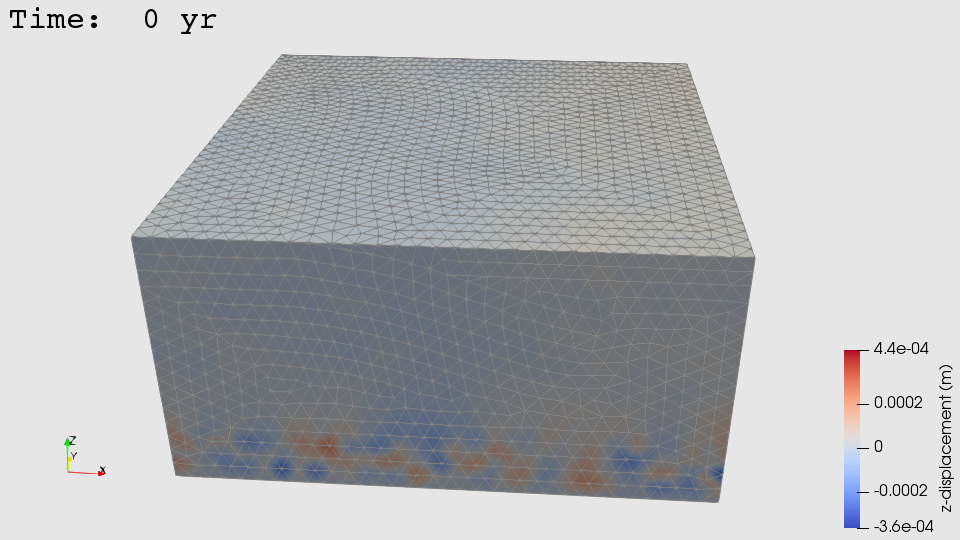
\includegraphics[height=6.1cm]{figs/subduction3d_step08b_soln}
  \end{center}
\vfill
      
\end{frame}


% ========================================================== SECTION
\subsection{Step 8c}

% ------------------------------------------------------------ SLIDE
\begin{frame}
  \frametitle{Step 8c}
  \summary{Viscoelastic finite strain with correct initial elastic stress}

  \vfill
  \begin{center}
      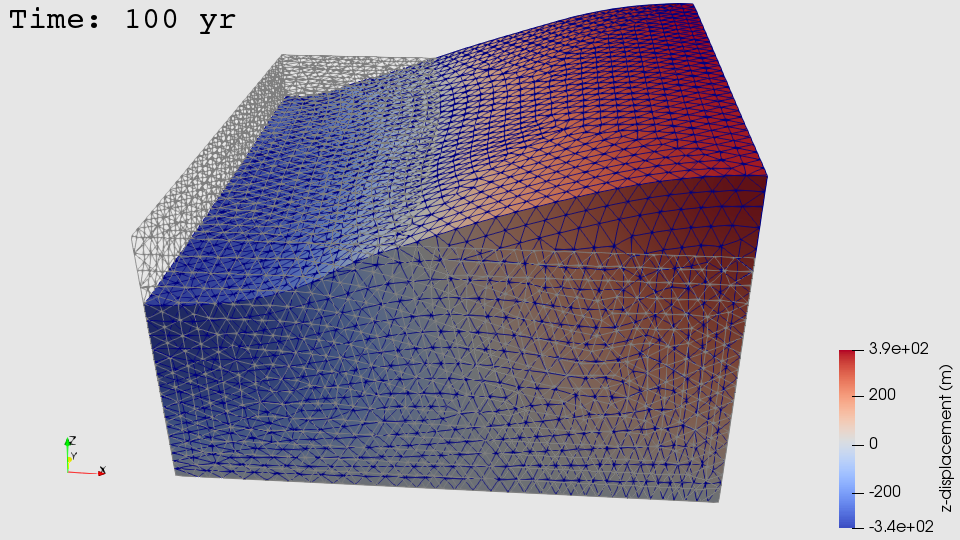
\includegraphics[height=6.1cm]{figs/subduction3d_step08c_soln}
  \end{center}
\vfill
      
\end{frame}


% ======================================================================
\end{document}


% End of file
